% Created 2014-12-23 Tue 17:09
\documentclass[11pt]{article}
\usepackage[utf8]{inputenc}
\usepackage[T1]{fontenc}
\usepackage{fixltx2e}
\usepackage{graphicx}
\usepackage{longtable}
\usepackage{float}
\usepackage{wrapfig}
\usepackage{rotating}
\usepackage[normalem]{ulem}
\usepackage{amsmath}
\usepackage{textcomp}
\usepackage{marvosym}
\usepackage{wasysym}
\usepackage{amssymb}
\usepackage{hyperref}
\tolerance=1000
\author{guifi.net community}
\date{\today}
\title{quick Mesh project (qMp.cat) workshop}
\hypersetup{
  pdfkeywords={},
  pdfsubject={},
  pdfcreator={Emacs 24.4.50.1 (Org mode 8.2.6)}}
\begin{document}

\maketitle
\tableofcontents


\section{Introduction}
\label{sec-1}
The basic material to deploy qMp cloud networks.

The radios used have Power over Ethernet (PoE) of 24V, it means that
the electrical power and data of the radio goes through an ethernet
cable. The blue cable in figure \ref{fig:poe} is what is deployed into an
outdoor place (typically rooftop or a balcony) where the qMp devices
will be installed and takes the POE interface in PoE injector. The
other interface in the PoE injector is LAN \footnote{LAN cable can make a length up to 100m if only is carrying data} and can be placed
to a PC or a switch/router if it is wanted to connect more
PC's. Finally, the PoE injector requires standard electrical
power. \textbf{Warning}: a PoE connection to a device that is not prepared to
work with PoE 24V, for example an ethernet interface of a computer,
can produce malfunction of its ethernet interface.

\begin{figure}[htb]
\centering
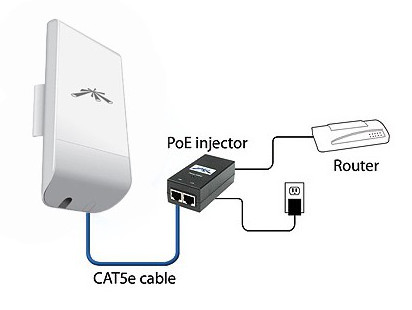
\includegraphics[width=.9\linewidth]{./img/general/poe.jpg}
\caption{\label{fig:poe}PoE network diagram}
\end{figure}

\section{Installer basics: Items}
\label{sec-2}
\begin{itemize}
\item Outdoor cable and rj45 connectors (sold separately) \\
  The cable should be for outdoor to resist the weather. 
\begin{itemize}
\item UTP cable: cable without protection. But sometimes it is enough.
\item FTP cable (recommended): cable with basic protection. ESD
prevention \footnote{\url{http://en.wikipedia.org/wiki/Electrostatic_discharge}}. The difference is that the cable has
ground.
\end{itemize}
\item Crimp tool: to join rj45 connector to cable.
\item Cable tester (recommended): a unexpensive one can help to work quickly and
reliably in the installation of cable.
\item Cable cutter: To take a segment of cable for a installation. Note:
UTP cable is easier to cut than FTP.
\item Cable tie: To lock the cable \& radio to a mast and other
cables.
\item Shopping cart or traveling bag with wheels (recommended): carry
all the items needed.
\item Measure meter: measure accurately the length of cable needed
(optional).
\end{itemize}
\section{Installer basics: 5GHz devices}
\label{sec-3}
The devices selected are working in the 5 GHz band because 2.4GHz is widely
used in cities and have more interferences. They are from Ubiquiti
manufacturer and compatible with qMp firmware.

\begin{description}
\item[{Unexpensive}] less than 100 euro.

\begin{description}
\item[{NanoStation Loco M5 (NSLM5)}] Short distances (less than
1km). The connection with the other candidate node has an
acceptable connection and there is no need to increase the
power signal of wifi. It uses the same firmware as
NanostationM5.
\item[{Nanostation M5 (NSM5)}] \footnote{\url{http://dl.ubnt.com/datasheets/nanostationm/nsm_ds_web.pdf}} If is needed a better connection to
specific node.
\item[{NanoBeam M5 different models}] \footnote{\url{http://ubnt.com/downloads/datasheets/nanobeam/NanoBeamM_DS.pdf}} When there is a long
distance connection (more than 1km). Use the same firmware as
NanostationM5. Is the evolution of NanoBridge M5 that is now
deprecated.
\end{description}

\item[{Expensive}] more than 100 euro.

\begin{description}
\item[{Rocket M5 }] \footnote{\url{http://ubnt.com/downloads/rocketM5_DS.pdf}} Base station to put different kind of antennas.
\begin{description}
\item[{Rocket M5 + Sector Antenna (S) 90 or 120 deg}] \footnote{\url{http://dl.ubnt.com/AirMax5GSectors.pdf}} when the need
is to cover a sector region with constant coverage of 90 or
120 deg. There are High Gain (HG) and Mid Gain (MG) versions.
\item[{Rocket M5 + Dish (D)}] \footnote{\url{http://ubnt.com/downloads/datasheets/rocketdish/rd_ds_web.pdf}} Longest distances (50km link \footnote{\url{http://blog.altermundi.net/article/completamos-el-enlace-de-50km/}}).
\end{description}
\end{description}
\end{description}

Summary of some relevant information at Table \ref{tab:devspec}:
\begin{table}[htb]
\caption{\label{tab:devspec}Devices specifications}
\centering
\begin{tabular}{lllllr}
Devices & Gain (dBi) & Beamwidth (deg) & Proc. & RAM & Flash\\
 &  & Hpol/Vpol/Elevation &  & (MB) & (MB)\\
\hline
NSLM5 & 13 & 45/45/45 & 24KC & 32 S & 8\\
NSM5 & 16 & 43/41/15 & 24KC & 32 S & 8\\
NBM5 & 16, 19, 22, 25 & see on datasheet & 74KC & 64 D & 8\\
RM5 S90 MG, HG & 17, 20 & see on datasheet & 24KC & 64 S & 8\\
RM5 S120 MG, HG & 16, 19 & see on datasheet & 24KC & 64 S & 8\\
RM5 D & 30, 34 & see on datasheet & 24KC & 64 S & 8\\
\end{tabular}
\end{table}

\begin{description}
\item[{Proc}] Processor Specs.
\begin{description}
\item[{24KC}] Atheros MIPS 24KC, 400MHz
\item[{74KC}] Atheros MIPS 74KC, 560MHz
\end{description}
\item[{RAM}] Type of RAM:
\begin{description}
\item[{S}] SDRAM
\item[{D}] DDR2
\end{description}
\end{description}
\section{Flash qMp node}
\label{sec-4}
Steps to flash a device with qMp firmware. It is assumed a GNU/Linux
Ubuntu/Debian computer:
\begin{enumerate}
\item Download the \textbf{Factory image} \footnote{\url{http://fw.qmp.cat/}} for a supported device that
has the factory operating system \footnote{\url{http://qmp.cat/Supported_devices}}. \textbf{Sysupgrade image} is for
OpenWRT or qMp nodes that want to upgrade. \textbf{Guifi image} has better
integration with guifi.net web.
\item Rename the downloaded file to \texttt{qmp.bin}.
\item Download the tftp packets with the system's repository. In
terminal: \texttt{\$ sudo apt-get install tftp-hpa}.
\item Disconnect the internet connection.
\item Open a terminal and put:
\begin{verbatim}
$ ping 192.168.1.20
\end{verbatim}
It will help to know when the antenna is in the reset mode.
\item Connect the equipments as shown in Figure \ref{fig:flashdiagram}.
\begin{figure}[htb]
\centering
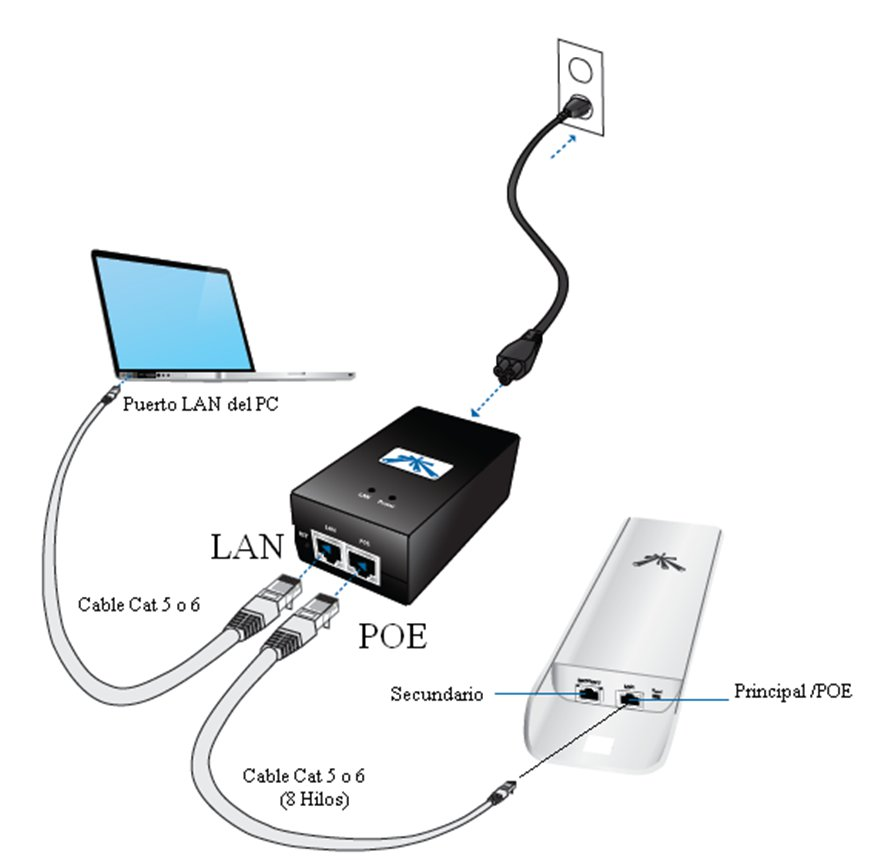
\includegraphics[width=.9\linewidth]{./img/general/flashdiagram.jpg}
\caption{\label{fig:flashdiagram}Network Diagram to Flash Antenna}
\end{figure}
\item Configure the network following one of these options:
\begin{enumerate}
\item \textbf{GUI option}: configure in the preferred network manager a
ethernet network with static IP in the computer to connect to
the device: \\
      IP: 192.168.1.10 \\
      Subnet: 192.168.1.100 \\
      Gateway: 192.168.1.1
\item \textbf{Terminal option}: 
\begin{verbatim}
$ sudo ip a a 192.168.1.25/24 dev eth0
\end{verbatim}
\end{enumerate}
\item Reset the device following one of these options:
\begin{enumerate}
\item \textbf{Reset in the antenna option}: Disconnect the interface of the
antenna. Remove the antenna's lid. With one hand take an object
with round toe, press and hold reset button (Figure
\ref{fig:resetant}) while with the other hand insert the ethernet
cable to the interface in antenna.
\begin{figure}[htb]
\centering
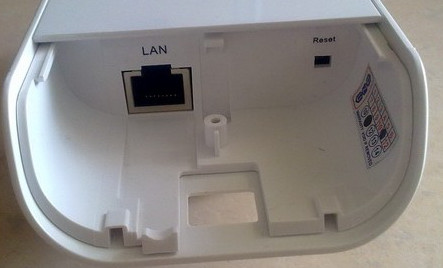
\includegraphics[width=.9\linewidth]{./img/general/reset-antenna.jpg}
\caption{\label{fig:resetant}Reset antenna}
\end{figure}
\item \textbf{Reset in the PoE injector option}: Check if the device has
PoE (Figure \ref{fig:resetpoe}). Disconnect the POE interface in PoE
injector. With one hand take an object with round toe, press and
hold reset button while with the other hand insert the ethernet
cable to the POE interface in PoE injector.
\begin{figure}[htb]
\centering
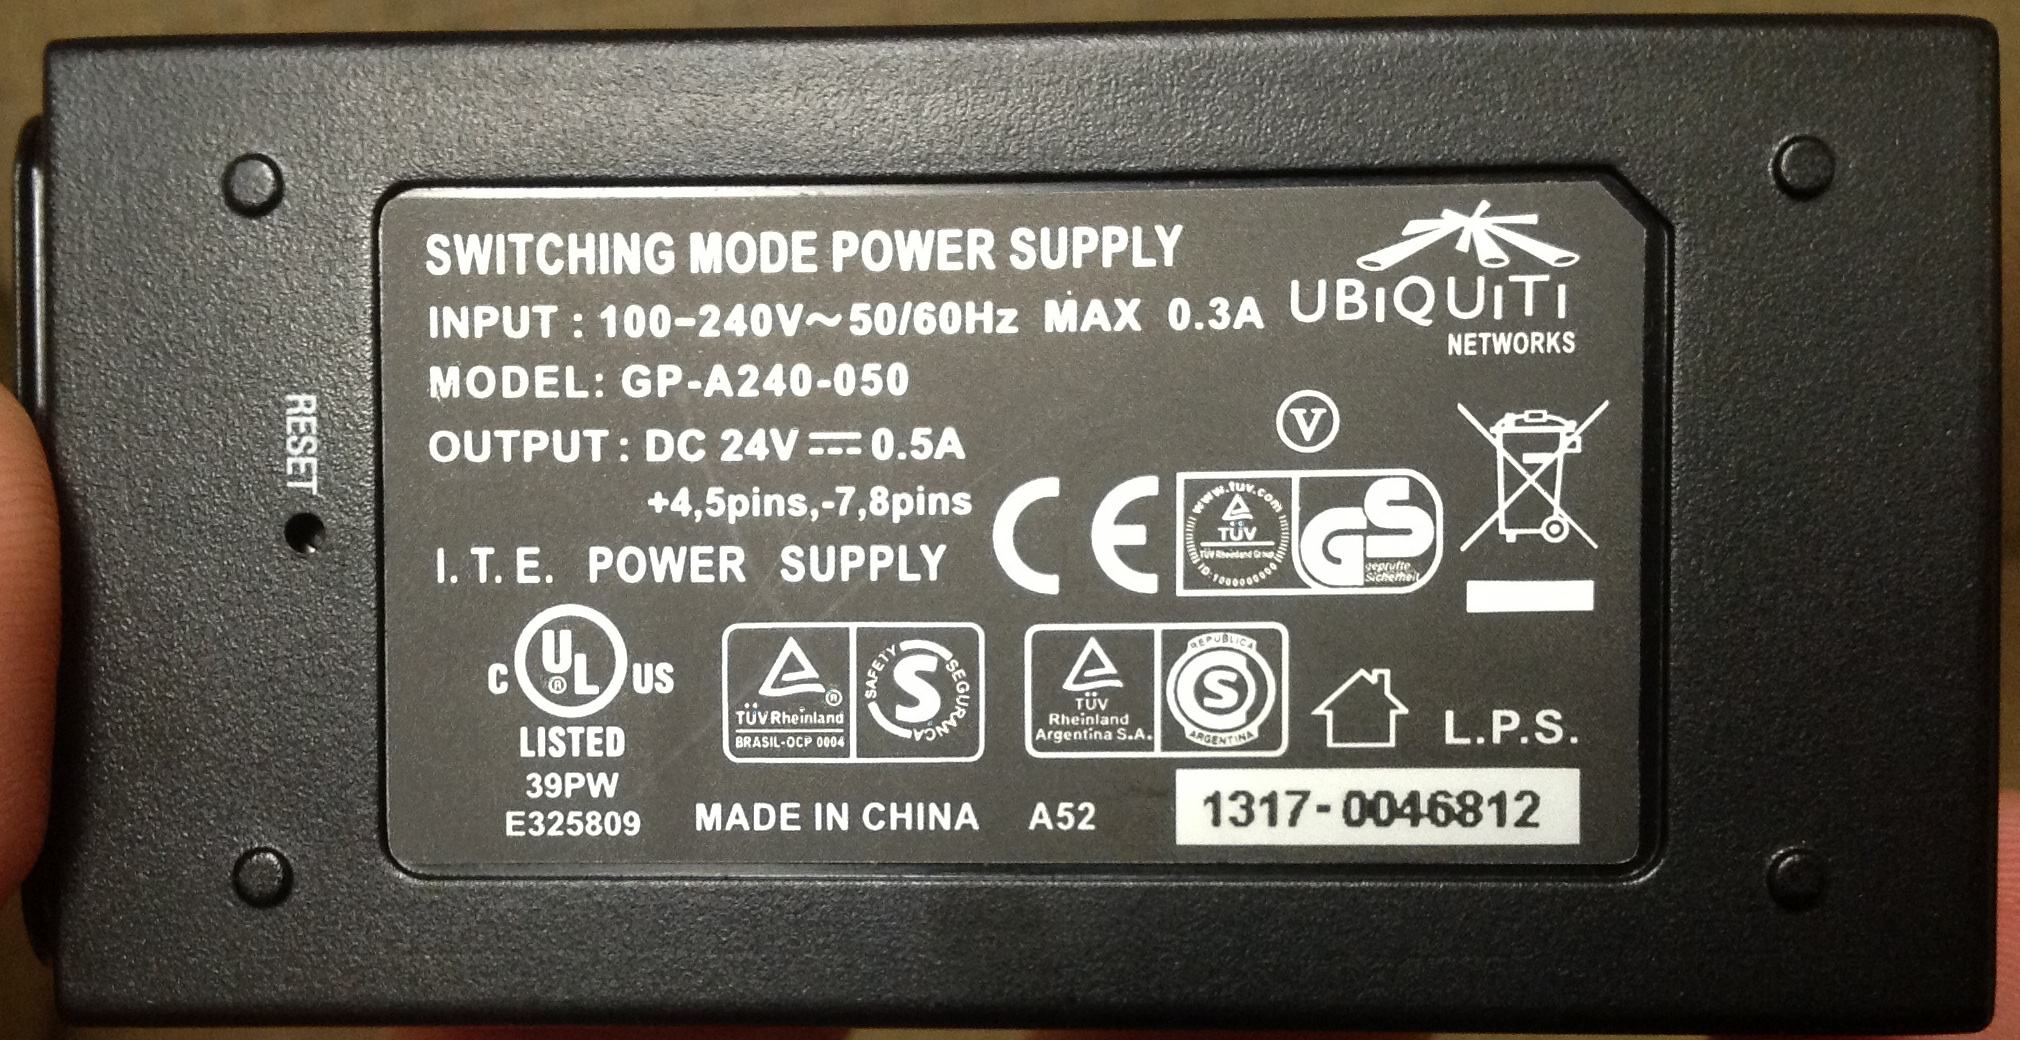
\includegraphics[width=.9\linewidth]{./img/general/reset-injector.jpg}
\caption{\label{fig:resetpoe}Reset power injector}
\end{figure}
\end{enumerate}
\item Observe if the antenna start the reset mode needed for continue:
\begin{itemize}
\item \textbf{Antenna led option}: Wait until the led 1 and 3 change to 2 and
4 cyclically. With this video resource it will give an idea of
time and led colors involved in the process \footnote{\url{https://www.youtube.com/watch?v=xIflE_-V-B4\#t=50s}}.
\item \textbf{PC screen option}: the ping starts responding. The output of the
\texttt{ping 192.168.1.20} should be something like:
\begin{verbatim}
64 bytes from X: icmp_req=X ttl=X time=X ms
\end{verbatim}
\end{itemize}
\item If is in reset mode stop pressing the reset button and put the
device in a stable place.
\item In a new terminal window, go where is the downloaded firmware
\texttt{qmp.bin}:
\begin{verbatim}
cd /path/to/the/qmpbin_folder
\end{verbatim}
And there, execute:
\begin{verbatim}
$ tftp 192.168.1.20
$ mode octet
$ trace
$ put qmp.bin
\end{verbatim}
[ Transmission process ]
\begin{verbatim}
$ quit
\end{verbatim}
\item After about 5 minutes, the 4th led of the ramp (the most right led,
Figure \ref{fig:ledsantenna}) is on, and not blinking. This is the moment to go the
next step.
\begin{figure}[htb]
\centering
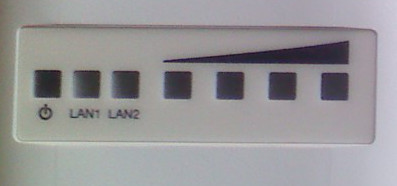
\includegraphics[width=.9\linewidth]{./img/general/blinkingled.jpeg}
\caption{\label{fig:ledsantenna}Led system in the antenna}
\end{figure}
\item Reconfigure the network to do a DHCP client in ethernet port
(Automatic IP) and try to connect again the PC with the device.
\item Check that the device responds to ping:
\begin{verbatim}
$ ping 172.30.22.1
\end{verbatim}
This is the fixed IP address in roaming mode. \\
    More general approach is to get the gateway address:
\begin{verbatim}
$ ip r | grep default | cut -f3 -d' '
\end{verbatim}
Open a web browser and check if this web can be accessed
(\textbf{Warning} admin.qmp it will only work if the PC is connected to
the device via DHCP):
\begin{verbatim}
http://admin.qmp
\end{verbatim}
alternatives:
\begin{verbatim}
http://172.30.22.1
http://<gateway_ip>
\end{verbatim}
\item Login access is
user: root \\
    password: 13f
\end{enumerate}

Other references \footnote{\url{http://wiki.ubnt.com/Firmware_Recovery}} \textsuperscript{,}\,\footnote{\url{http://www.qmp.cat/\#Use-the-firmware}} \textsuperscript{,}\,\footnote{tftp info: \url{http://wiki.openwrt.org/doc/howto/generic.flashing.tftp}}
\section{qMp basics: Testing operations}
\label{sec-5}
Figure \ref{fig:wan-status-on} shows the first screen obtained when there is
a log in a qMp node.

\begin{figure}[htb]
\centering
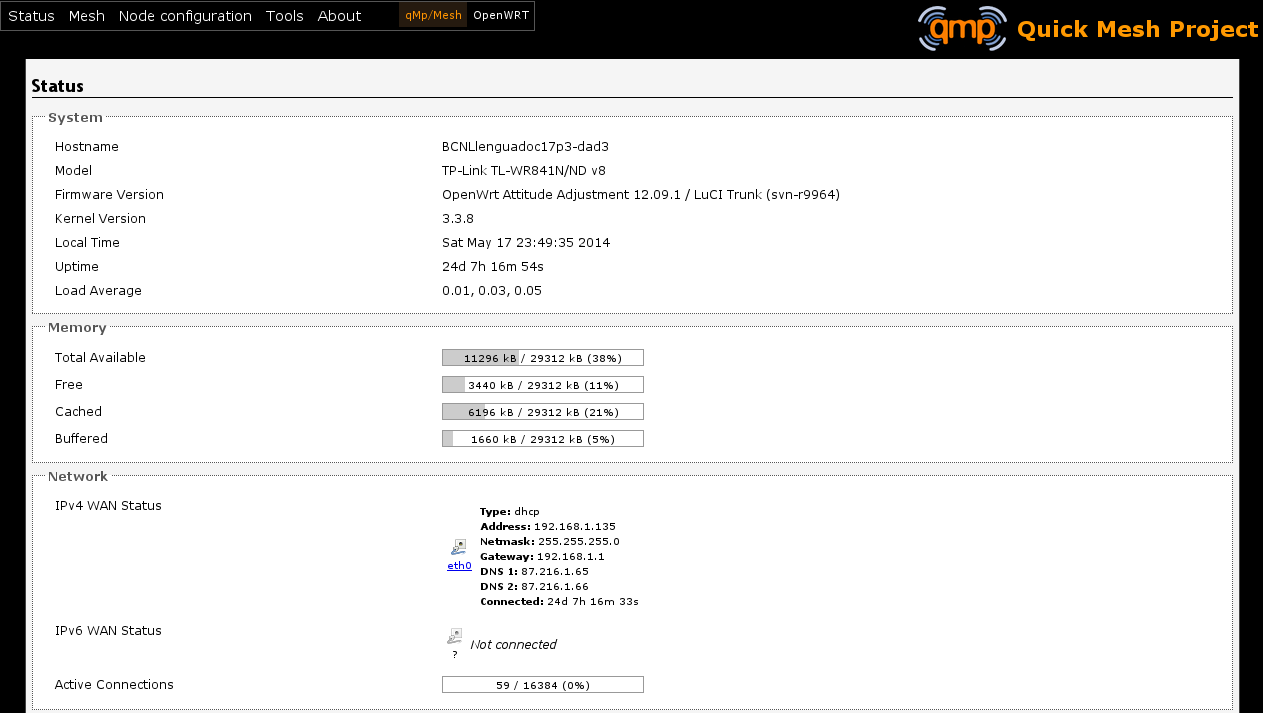
\includegraphics[width=.9\linewidth]{./img/qMp-basics-scrot/status-wan_status.png}
\caption{\label{fig:wan-status-on}First screen}
\end{figure}

\noindent
To come back to this screen, go to the menu clicking at:
\begin{verbatim}
qMp/Mesh / Status
\end{verbatim}
alternatively:\\
\url{http://admin.qmp/cgi-bin/luci/qmp/status}

When there is a scroll down action, appears Associated
Stations. Figure \ref{fig:associated-stations} has the wifi links with other
qMp nodes and what signal associated (dBm). The guifi.net good
practices says that the backbone should be better than
-75dBm \footnote{Catalan: \url{http://guifi.net/ca/BonesPractiquesUER}}. In that figure there are different kind of links with
different qualities. Good quality means high parameters of: dBm, RX
Rate, TX Rate [bandwidth (Mbps)] and MCS codification (the number).

These qualities refer to connection to different nodes, only is
shown the MAC address. But the MAC is enough to identify a node,
because the last four characters are appended in every hostname of the
network. Later, it will be known how to navigate to different nodes in the
network.

\begin{figure}[htb]
\centering
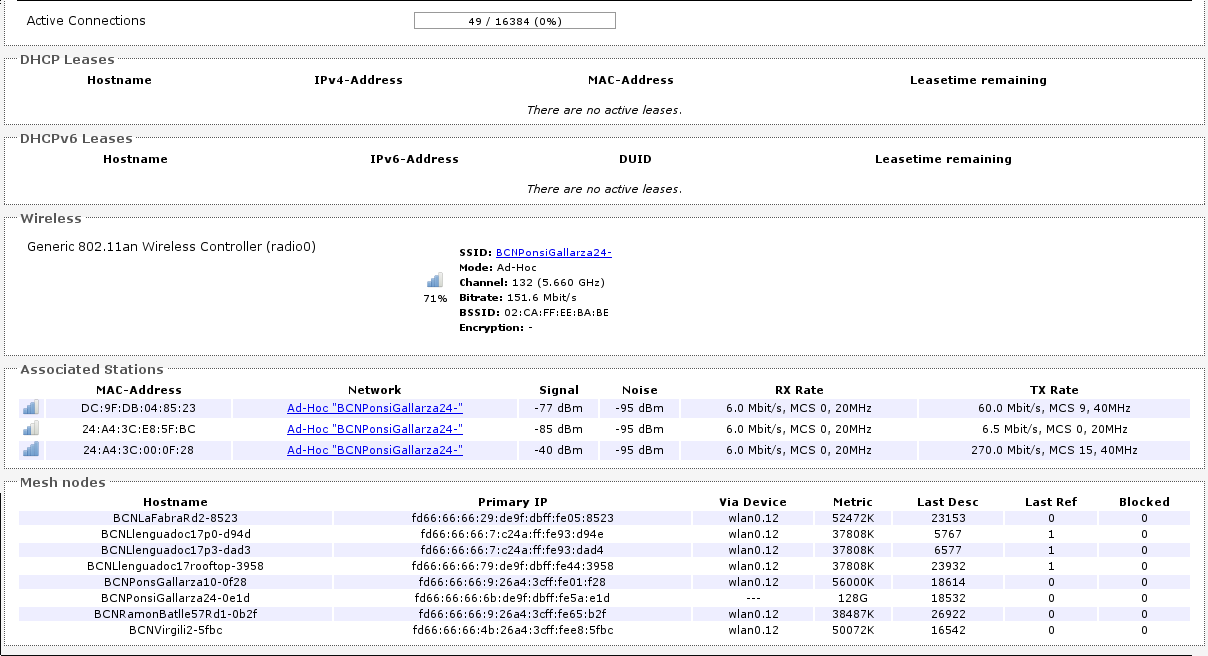
\includegraphics[width=.9\linewidth]{./img/qMp-basics-scrot/status-associated-nodes.png}
\caption{\label{fig:associated-stations}Associated stations}
\end{figure}

Another measure of quality is shown on Figure \ref{fig:links-node}. This is the
quality in terms of the protocol bmx6. A 0-100 rating in terms of
reception and transmission (rx/tx).

\noindent
To arrive there, go to the menu clicking at:
\begin{verbatim}
qMp/Mesh / Mesh / Links
\end{verbatim}
alternatively:\\
\url{http://admin.qmp/cgi-bin/luci/qmp/mesh/links}

\begin{figure}[htb]
\centering
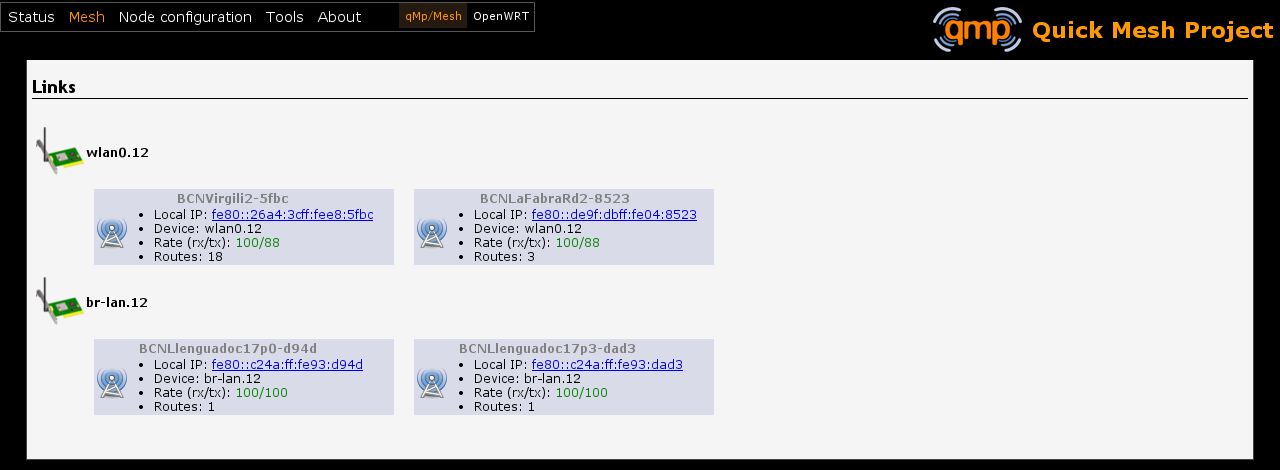
\includegraphics[width=.9\linewidth]{./img/qMp-basics-scrot/links.png}
\caption{\label{fig:links-node}Links of the node}
\end{figure}

Also, can be made a bandwidth test between nodes. Figure \ref{fig:bw-test}
perform a TCP connection benchmark and give the Mbps between the node
and other possible destinations. Wait until a single test ends to know
all the bandwidth in the link or route.

\noindent
To arrive there, go to the menu clicking at:
\begin{verbatim}
qMp/Mesh / Tools
\end{verbatim}
alternatively:\\
\url{http://admin.qmp/cgi-bin/luci/qmp/tools}

\begin{figure}[htb]
\centering
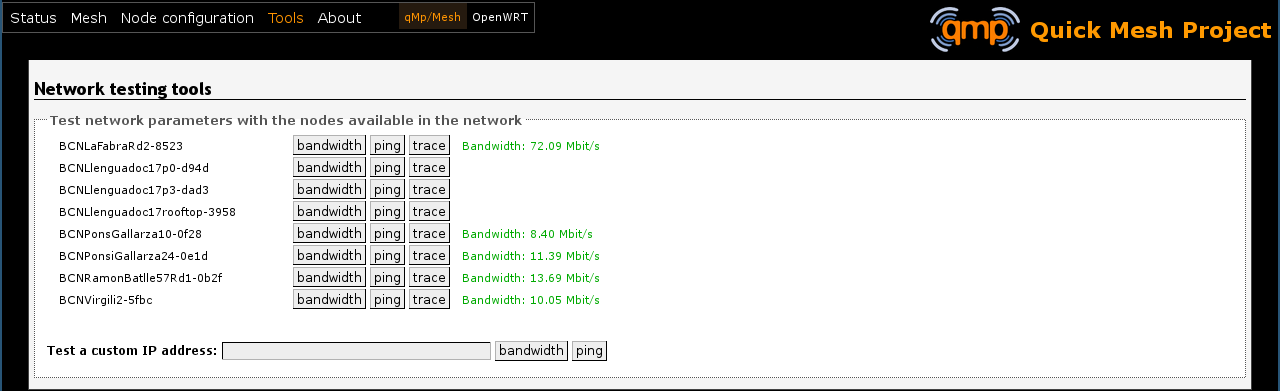
\includegraphics[width=.9\linewidth]{./img/qMp-basics-scrot/test-bandwidth.png}
\caption{\label{fig:bw-test}Bandwidth Test}
\end{figure}

Figure \ref{fig:wifi-signal-rt}. After the general scan, when there is a
node candidate to do a durable connection, there is the need to
analyse the quality of this link in real-time. This helps to select an
optimised place to lock the antenna in the installation.

\noindent
To arrive there, go to the menu clicking at:
\begin{verbatim}
OpenWRT / Status / Realtime Graphs / Wireless
\end{verbatim}
alternatively:\\
\url{http://admin.qmp/cgi-bin/luci/admin/status/realtime/wireless}

\begin{figure}[htb]
\centering
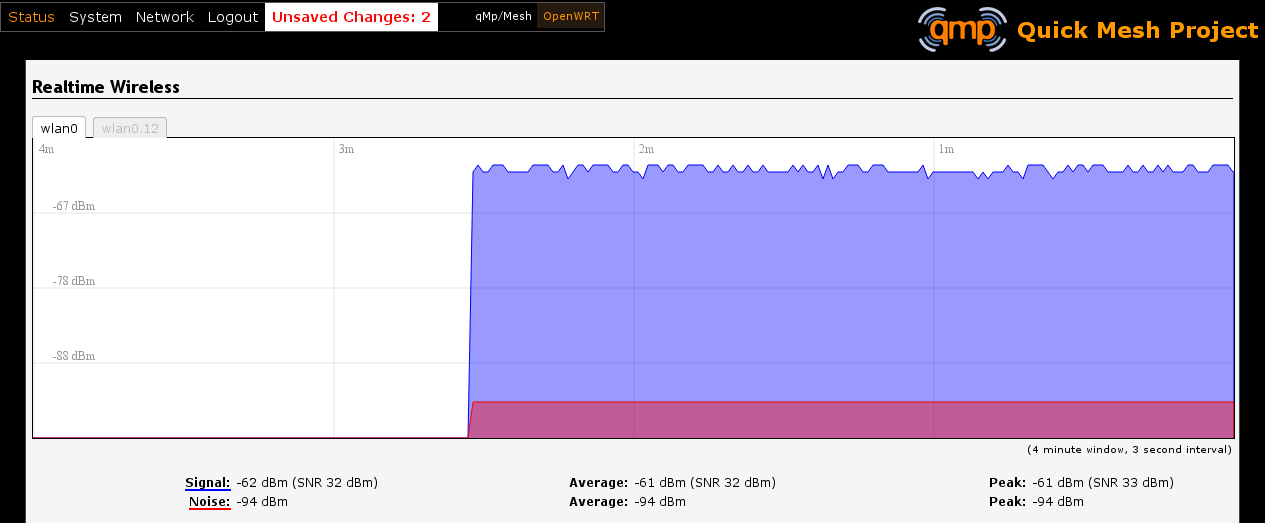
\includegraphics[width=.9\linewidth]{./img/qMp-basics-scrot/realtime_wifi_link.png}
\caption{\label{fig:wifi-signal-rt}Strength of the best wifi signal in real-time}
\end{figure}

The situation could be that cannot be a connection to the node to the
network. Perhaps it is in another channel. Figure \ref{fig:find-qmp} shows a
wifi scan. qMp always use BSSID: \texttt{02:CA:FF:EE:BA:BE}, in Mode
\texttt{Ad-Hoc}. These are two solid references to find other qMp networks. In
the figure there are two qMp networks in channels: 140 and 132.

\noindent
To arrive there, go to the menu clicking at:
\begin{verbatim}
OpenWRT / Network / Wifi / "Scan"
\end{verbatim}
alternatively:\\
\url{http://admin.qmp/cgi-bin/luci/admin/network/wireless}
and click Scan.

\begin{figure}[htb]
\centering
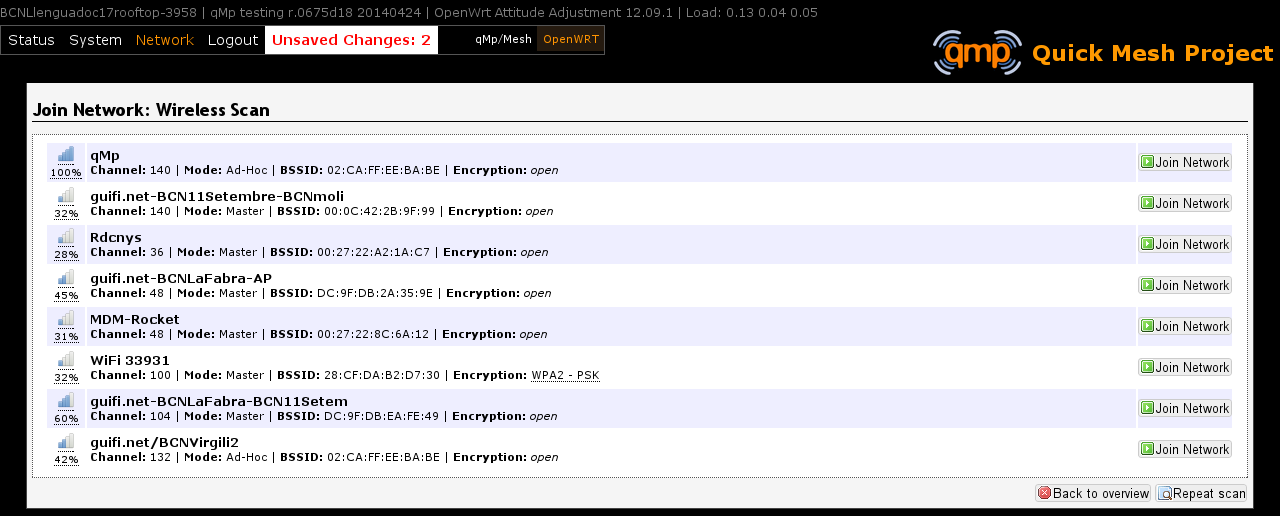
\includegraphics[width=.9\linewidth]{./img/qMp-basics-scrot/wifi_scan_find_qmp.png}
\caption{\label{fig:find-qmp}Wifi scan: find qMp network}
\end{figure}

If there is a design of a new qMp network it is important to select a
channel that is not used. Figure \ref{fig:interference} shows how another AP
is also using channel 140.

\begin{figure}[htb]
\centering
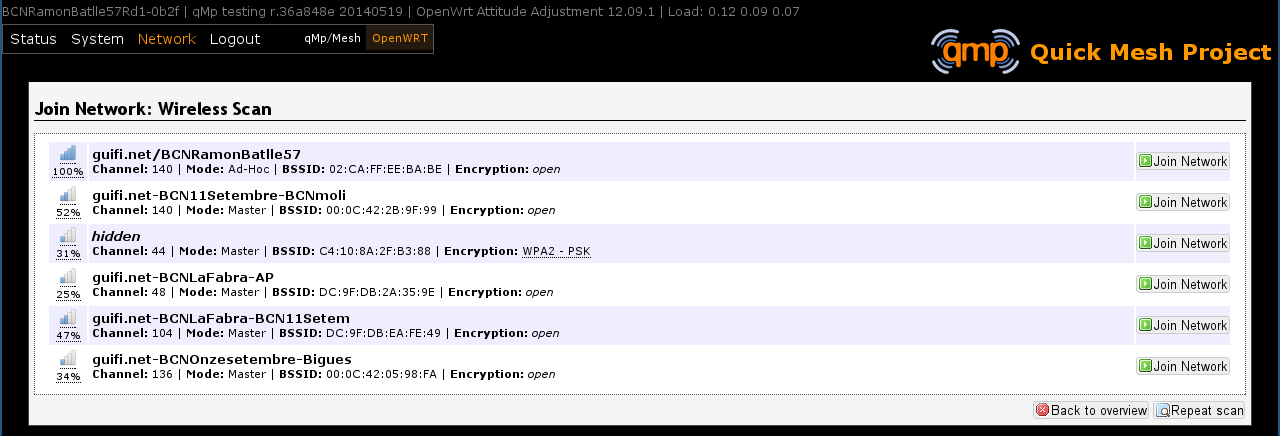
\includegraphics[width=.9\linewidth]{./img/qMp-basics-scrot/wifi_scan_interference.png}
\caption{\label{fig:interference}Wifi scan interference}
\end{figure}

Figure \texttt{wifi-channel-power} shows where to change wifi parameters as
wifi channel and power signal to the qMp network. By default, qMp uses
17, but it can be increased to 22 (max value).

Use the transmission power of wifi signal with care, in the interested
network is a communication signal, but for the other networks it is
another noise in the environment that make its communications more
difficult.

\noindent
To arrive there, go to the menu clicking at:
\begin{verbatim}
OpenWRT / Node configuration / Wireless Settings
\end{verbatim}
alternatively:\\
\url{http://admin.qmp/cgi-bin/luci/qmp/configuration/wifi/}

\begin{figure}[htb]
\centering
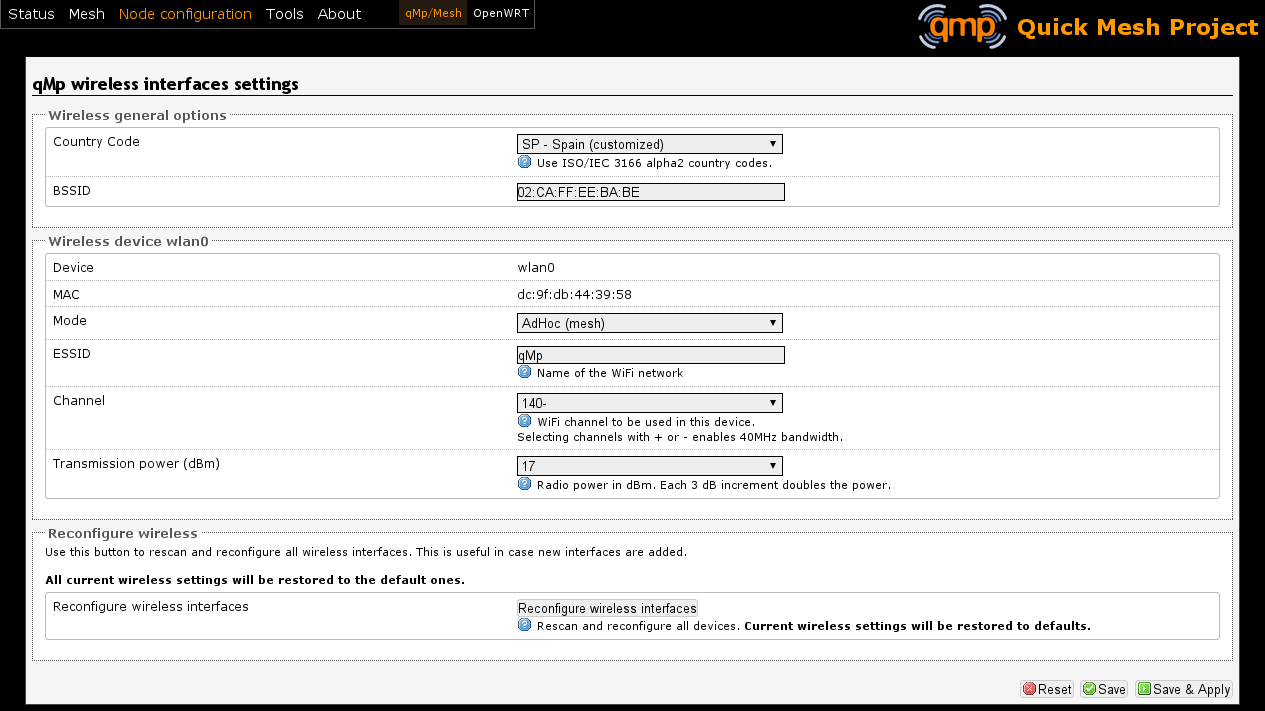
\includegraphics[width=.9\linewidth]{./img/qMp-basics-scrot/wifi-channel-power.png}
\caption{\label{fig:wifi-channel-power}Wifi: Channel \& Power}
\end{figure}

Figure \ref{fig:tunnels} (marked as red) shows that there is a WAN Node, the
node makes announcement of this network as \texttt{Internet}. If can be
arrived there, it means there is an internet connection, try it with a
browser. Also could be interesting to perform additional bandwidth
tests \footnote{\url{http://www.catnix.net/en/speedtest}} \textsuperscript{,}\,\footnote{\url{http://speedtest.net}} \textsuperscript{,}\,\footnote{\url{http://testdevelocidad.es}} \textsuperscript{,}\,\footnote{\url{http://testvelocidad.eu/}}.

But perhaps the WAN node cannot be accessed, or there is not a WAN
node in the network. Can be checked if there is a tunnel to Internet.

In the same view, can be browsed for a Border Node. Figure
\ref{fig:tunnels} shows it (marked as blue), the node makes announcement of
the network \texttt{10.0.0.0/8}, it means, access to the rest of guifi.net

\noindent
To arrive there, go to the menu clicking at:
\begin{verbatim}
qMp/Mesh / Mesh / Tunnels
\end{verbatim}
alternatively:\\
\url{http://admin.qmp/cgi-bin/luci/qmp/Mesh/Tunnels}

\begin{figure}[htb]
\centering
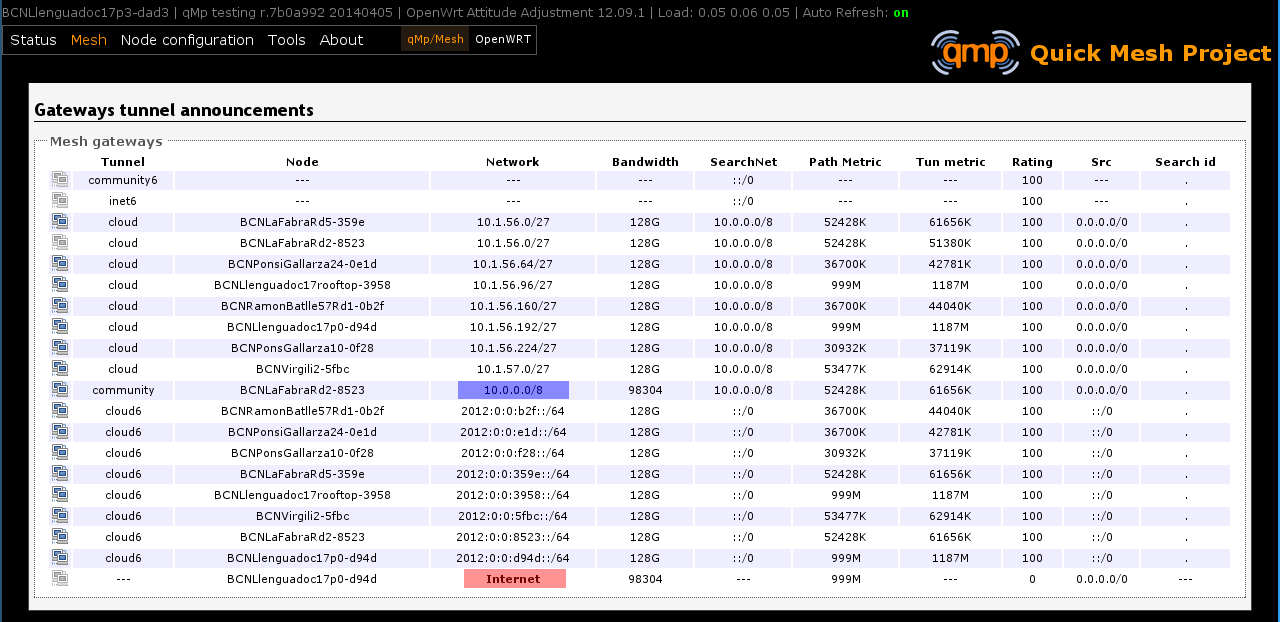
\includegraphics[width=.9\linewidth]{./img/qMp-basics-scrot/tunnels.png}
\caption{\label{fig:tunnels}Tunnels}
\end{figure}

\section{qMp basics: Basic install and maintaining}
\label{sec-6}
Figure \ref{fig:quick-setup}, this is the final setup when the node is
prepared to be in testing phase.

In guifi.net web page, after adding the device, it is received a unique ip
address, and is needed a \texttt{255.255.255.244} netmask. Use the same name
as in the web or the network organization page.

\noindent
To arrive there, go to the menu clicking at:
\begin{verbatim}
qMp/Mesh / Node configuration / qMp easy setup
\end{verbatim}
alternatively:\\
\url{http://admin.qmp/cgi-bin/luci/qmp/configuration/easy_setup/}

\begin{figure}[htb]
\centering
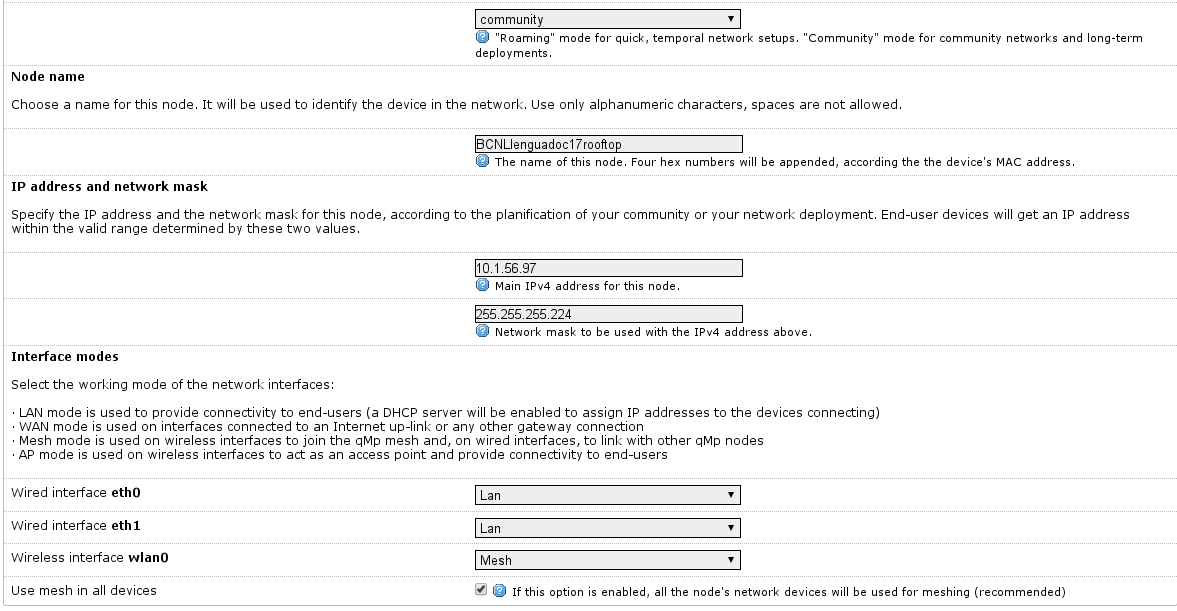
\includegraphics[width=.9\linewidth]{./img/qMp-basics-scrot/quick_setup.png}
\caption{\label{fig:quick-setup}Quick setup}
\end{figure}

Figure \ref{fig:backup}: When the node is working fine is important to make
a backup of the configuration. It is not recommended to upgrade the
node using this menu for the qMp firmware.

\noindent
To arrive there, go to the menu clicking at:
\begin{verbatim}
OpenWRT / System / "Backup/Flash Firmware"
\end{verbatim}
alternatively:\\
\url{http://admin.qmp/cgi-bin/luci/admin/system/flashops}

\begin{figure}[htb]
\centering
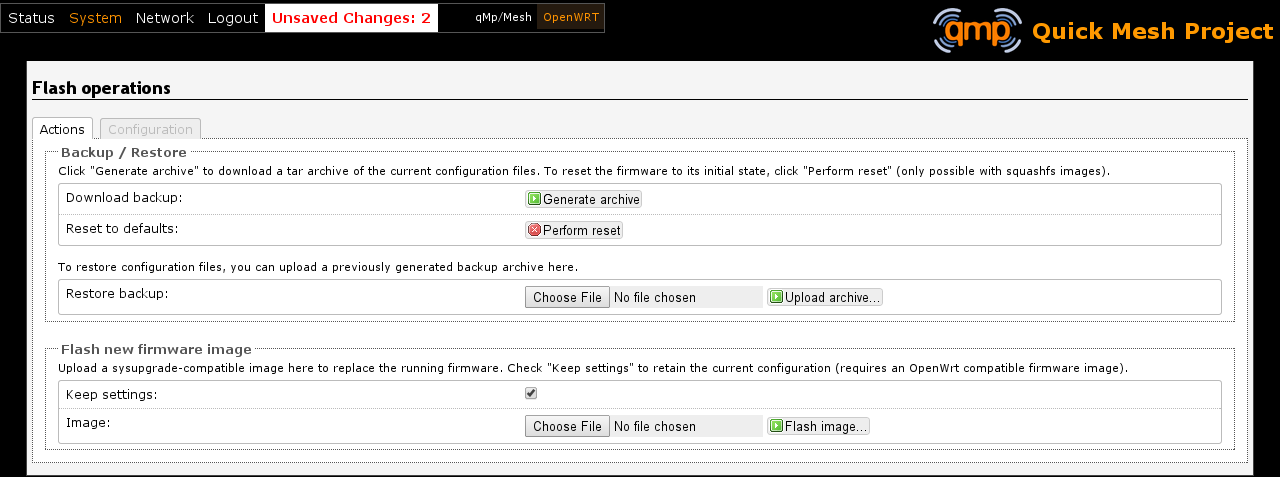
\includegraphics[width=.9\linewidth]{./img/qMp-basics-scrot/backup-new-firmware.png}
\caption{\label{fig:backup}Backup}
\end{figure}

For upgrade the node at the moment it is only possible via
terminal. Do a login with ssh session:
\begin{verbatim}
ssh root@admin.qmp
\end{verbatim}
password: 13f \\
From this point, there are three methods:
\begin{enumerate}
\item Automatic upgrade (with internet connection in the node).
\begin{verbatim}
qmpcontrol upgrade
\end{verbatim}
\item Upgrade with a link (with internet connection in the node).
\begin{verbatim}
qmpcontrol upgrade "http://...qmp.bin"
\end{verbatim}
It means the URL where is located the qMp firmware, remember that
can be found all the firmwares supported here: \url{http://fw.qmp.cat}
\item Upgrade with a local file (without internet connection in the node).
\begin{enumerate}
\item Put the file inside qMp node, open a new terminal and put
\begin{verbatim}
scp qmp.bin root@admin.qmp:/tmp
\end{verbatim}
It will ask for the password
\item With the existing ssh session opened before, or a new one,
login with ssh and:
\begin{verbatim}
qmpcontrol upgrade "/tmp/qmp.bin"
\end{verbatim}
\end{enumerate}
\end{enumerate}
Confirm to continue with the upgrade process and wait until it is finished.

Note: qMp only save common settings after the upgrade, concretely:
\begin{verbatim}
# cat /etc/config/qmp | grep preserve
\end{verbatim}

For other file changes, perform a backup before the upgrade.
\section{qMp basics: Navigating inside the network}
\label{sec-7}
Figure \ref{fig:net-nodes} shows a screen that presents all the qMp nodes
conforming the cloud. By clicking the blue spherical icon to the left
of each node it is possible to obtain additional information about
them. In particular, the network address announced by one node can be
found under the \texttt{Gateways announced} label, and the IP of the node in
the first address of that network. In the example shown in the figure,
the network address is \texttt{10.1.56.96} and the IP of the qMp node is
\texttt{10.1.56.97}.

\noindent
To arrive there, go to the menu clicking at:
\begin{verbatim}
qMp/Mesh / Mesh / Nodes
\end{verbatim}
alternatively:\\
\url{http://admin.qmp/cgi-bin/luci/qmp/mesh/nodes}

\begin{figure}[htb]
\centering
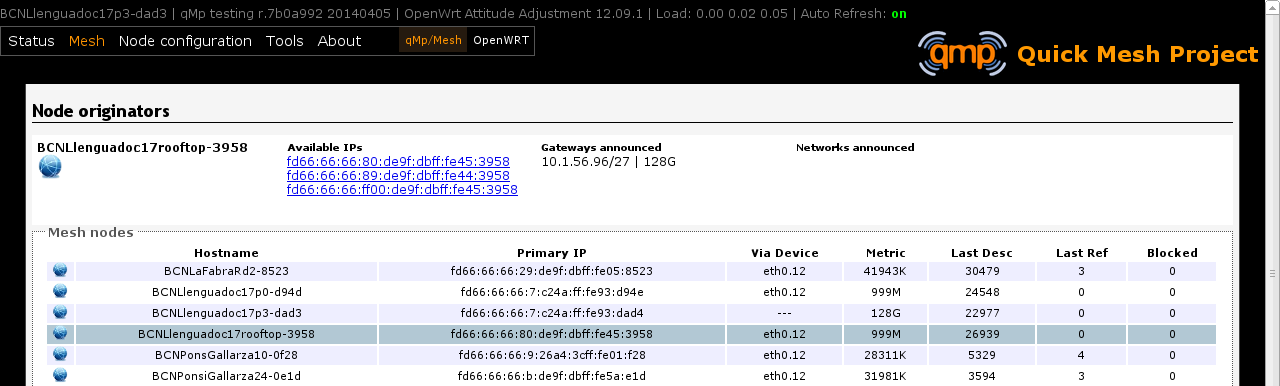
\includegraphics[width=.9\linewidth]{./img/qMp-basics-scrot/net-of-nodes.png}
\caption{\label{fig:net-nodes}IP address of nodes}
\end{figure}

Figure \ref{fig:graph-network} is the graph that shows the nodes, the edges
with the bmx6's quality rate show how each are connected.

\noindent
To arrive there, go to the menu clicking at:
\begin{verbatim}
qMp/Mesh / Mesh / Graph
\end{verbatim}
alternatively:\\
\url{http://admin.qmp/cgi-bin/luci/qmp/mesh/graph}

\begin{figure}[htb]
\centering
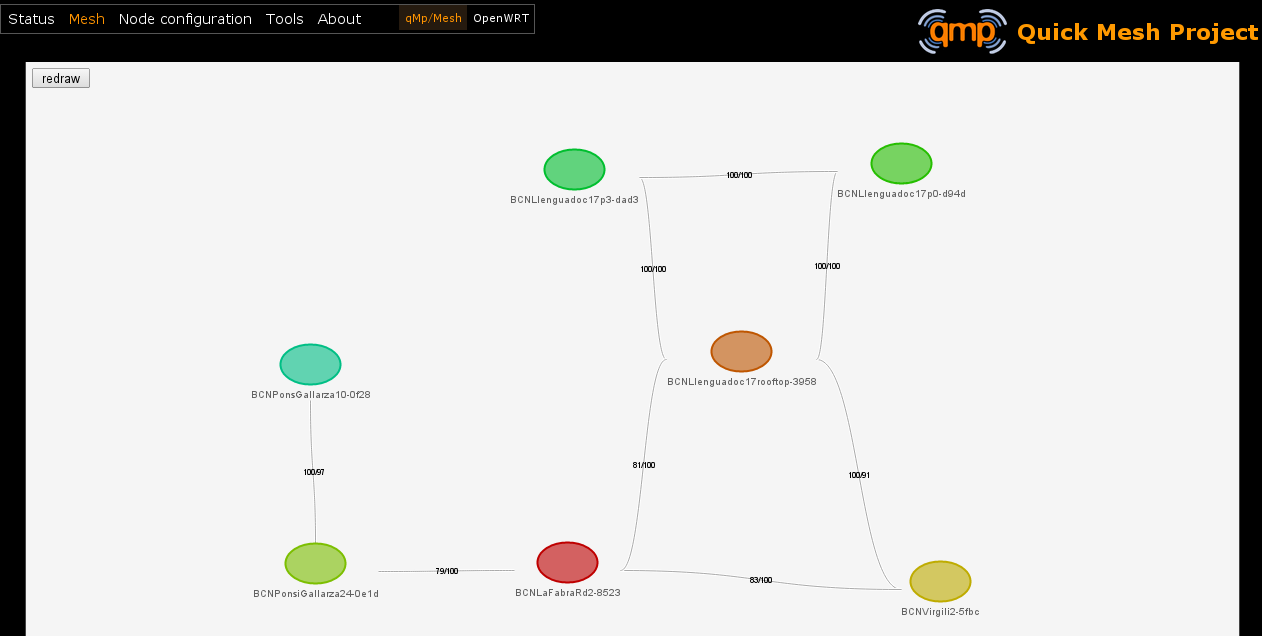
\includegraphics[width=.9\linewidth]{./img/qMp-basics-scrot/graph.png}
\caption{\label{fig:graph-network}Graph of the network}
\end{figure}
\section{Proposed qMp cloud node designs: WAN node design}
\label{sec-8}
To build a WAN node, figure \ref{fig:wan-gen} shows how the qMp node should
be connected to the \emph{mesh} network (through wifi via bmx6 routing) and
Internet (through ethernet to ISP \footnote{Internet Service Provider} router via DCHP client).

It is recommended to use the device Nanostation M5 because it has two
ethernet interfaces (eth0, eth1). With one can be made a DHCP server
to connect to the qMp node with a laptop. And for the other ethernet,
a DHCP client to the ISP router.

In the case that there is a Nanostation Loco M5, it only has one
ethernet (eth0 \footnote{eth1 is ignored}). It will be for the DHCP client to the ISP
router and it means that there is no DHCP server to directly connect
to the qMp node. An easy solution is that the connection to the qMp
node could be possible with another qMp node in the network (it is
being used the wifi interface).

\begin{figure}[htb]
\centering
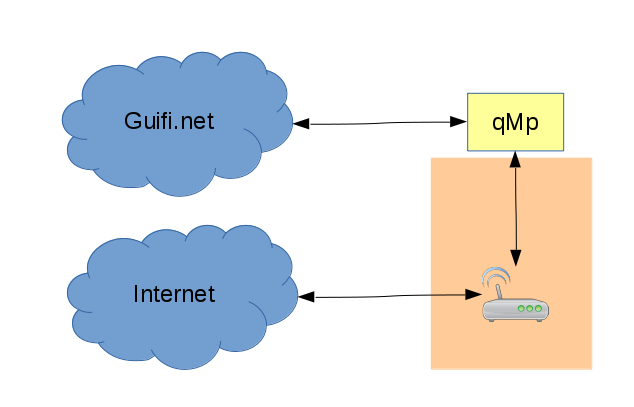
\includegraphics[width=.9\linewidth]{./img/mesh-designs/wan_node_generic.png}
\caption{\label{fig:wan-gen}Network diagram generic WAN node}
\end{figure}

To set the ethernet that will do the DHCP client to the ISP router
there are 2 options.

Option 1: in the quick setup, last part says what to do with
interfaces (figure \ref{fig:quickdhcp}). The interfaces have 3 selections:
\texttt{Mesh}, \texttt{Lan} (DHCP server) and \texttt{WAN} (DHCP client).

\begin{figure}[htb]
\centering
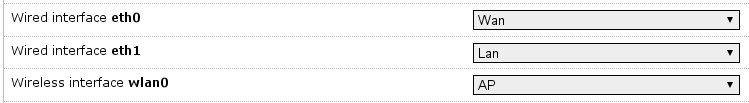
\includegraphics[width=.9\linewidth]{./img/qMp-basics-scrot/quick_setup_interfaces.png}
\caption{\label{fig:quickdhcp}Option 1: Set DHCP client to interface with quick setup}
\end{figure}

Option 2: Figure \ref{fig:netset} shows the screen that set the DHCP client
interface, and there is no need to do a quick setup with the node.

\noindent
To arrive there, go to the menu clicking at:
\begin{verbatim}
OpenWRT / Node configuration / Network Settings
\end{verbatim}
alternatively:\\
\url{http://admin.qmp/cgi-bin/luci/qmp/configuration/network/}

\begin{figure}[htb]
\centering
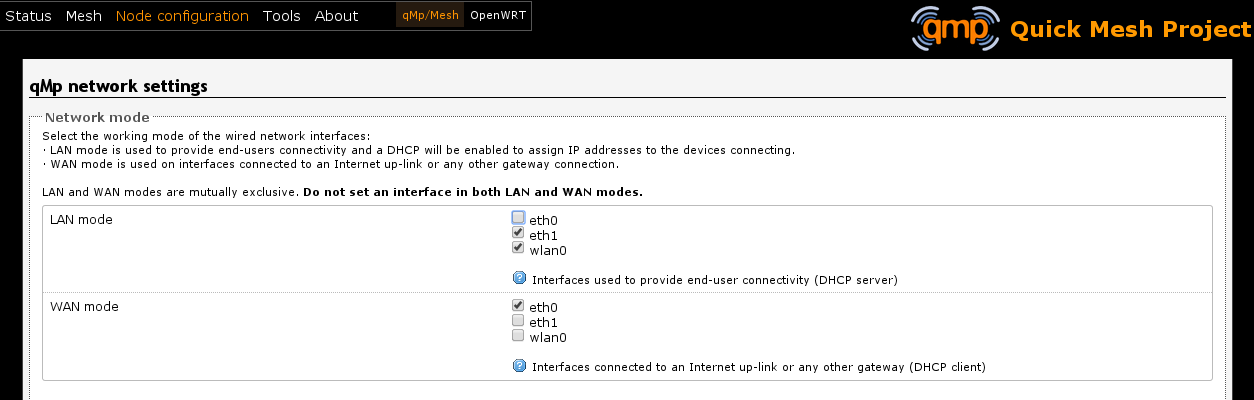
\includegraphics[width=.9\linewidth]{./img/qMp-basics-scrot/network_settings.png}
\caption{\label{fig:netset}Option 2: Set DHCP client to interface with network settings}
\end{figure}

To test that is working the DHCP client to the ISP router, check the
IPv4 WAN Status, section Network. Figure \ref{fig:wan-status-on-detail} shows a
successful WAN connection. Figure \ref{fig:wan-status-off} shows a
unsuccessful WAN connection: there is no DHCP client or is not
correctly connected.

\begin{figure}[htb]
\centering
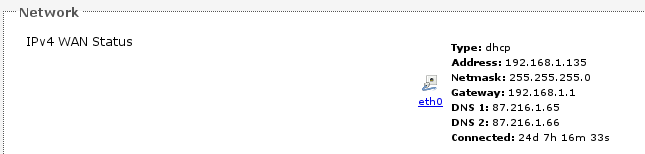
\includegraphics[width=.9\linewidth]{./img/qMp-basics-scrot/status-wan_status_detail.png}
\caption{\label{fig:wan-status-on-detail}WAN status online}
\end{figure}

\begin{figure}[htb]
\centering
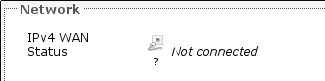
\includegraphics[width=.9\linewidth]{./img/qMp-basics-scrot/wan_not_connected.png}
\caption{\label{fig:wan-status-off}WAN status offline}
\end{figure}

\noindent
To arrive there, go to the menu clicking at:
\begin{verbatim}
qMp/Mesh / Mesh / Status
\end{verbatim}
alternatively:\\
\url{http://admin.qmp/cgi-bin/luci/qmp/status}
\section{Proposed qMp cloud node designs: General node design}
\label{sec-9}
Figure \ref{fig:gen-node} shows the elements of a simple node installation:
A qMp node connected to its network and a 2.4 GHz wifi router as an
Access Point that it is necessary to give wifi coverage inside the
place.
\begin{figure}[htb]
\centering
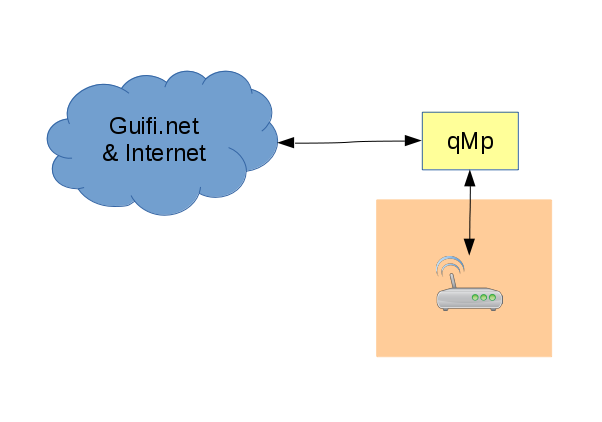
\includegraphics[width=.9\linewidth]{./img/mesh-designs/generic_node.png}
\caption{\label{fig:gen-node}Network diagram generic node}
\end{figure}
\section{Making a panorama with Hugin}
\label{sec-10}
With Hugin it is very easy to do panorama photos, and is free open
source software \footnote{\url{http://hugin.sourceforge.net/}}.

\begin{enumerate}
\item How to do the photos? Take the same physical point and start doing
photos with 20\% of overlap between them.
\item Follow the steps in Hugin's program (Figure: \ref{fig:hugin})
\begin{enumerate}
\item \texttt{1.Load images}, select all images in the folder it is wanted to
do a panorama.
\item \texttt{2.Align}.
\begin{itemize}
\item this takes a process to search for control points for give
sensation of continuity in the photo.
\item if there is not enough control points, search
control points manually or do the photos again.
\end{itemize}
\item \texttt{3.Create panorama}: save a .pto and .tiff files in the folder with
all images.
\end{enumerate}
\begin{figure}[htb]
\centering
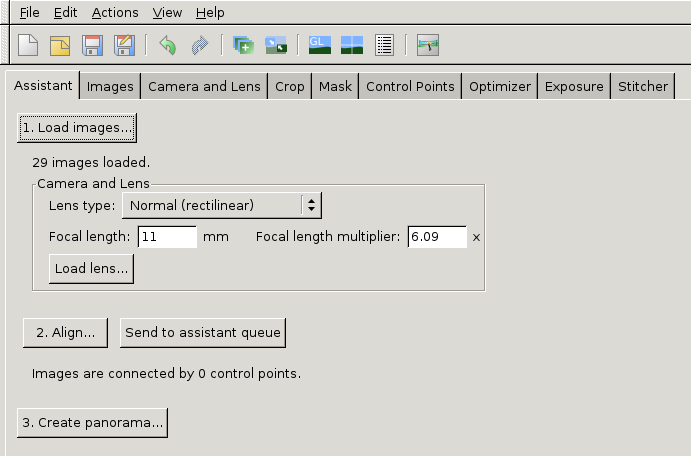
\includegraphics[width=.9\linewidth]{./img/general/hugin.png}
\caption{\label{fig:hugin}Hugin}
\end{figure}
\item Conversion of .tiff to .jpeg \\
   If it is wanted to share the panorama.
\begin{verbatim}
sudo apt-get install imagemagick
convert pan.tiff pan.jpeg
\end{verbatim}
An example is showed in figure \ref{fig:exhugin}
\begin{figure}[htb]
\centering
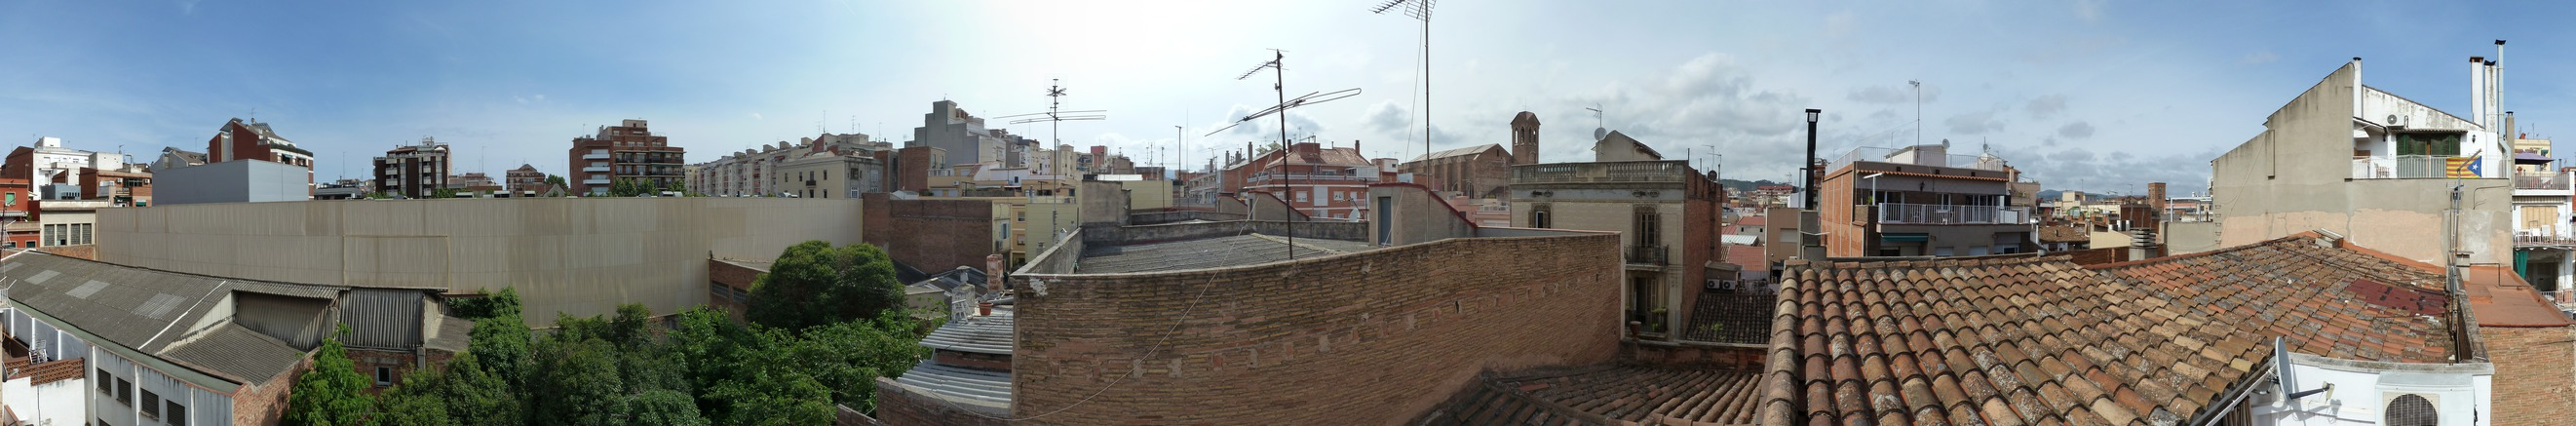
\includegraphics[width=.9\linewidth]{./img/santandreudeploy/llenguadoc.jpg}
\caption{\label{fig:exhugin}Example of panorama using hugin}
\end{figure}
\end{enumerate}

\section{About monitoring}
\label{sec-11}
Perform a monitoring of the network is important as a measure of
quality assurance. Are presented 3 alternatives.
\subsection{\textbf{From the guifi web}}
\label{sec-11-1}
can be obtained the graphs. It helps to know if the device is up, its
ping and the network traffic. Figure \ref{fig:snpservices} shows how it
looks like.

\begin{figure}[htb]
\centering
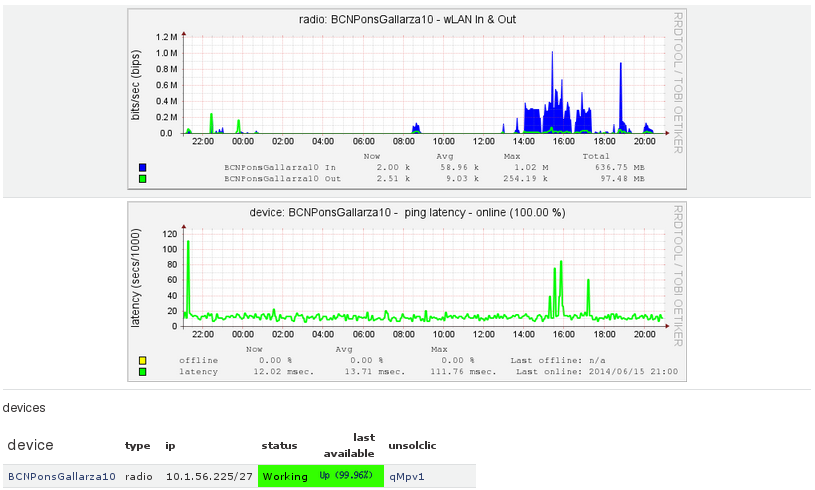
\includegraphics[width=.9\linewidth]{./img/general/snpservices.png}
\caption{\label{fig:snpservices}Graph server in guifi.net}
\end{figure}

It is required a qMp version with guifi package: \texttt{qMp-Guifi} should
appear in the bin package name.

The server part uses a package developed by guifi.net community called
\texttt{snpservices}. For install it can be followed this guide \footnote{There is no English translation: \url{http://ca.wiki.guifi.net/wiki/Servidor_de_gr\%C3\%A0fiques_1}},
basically, a Debian repository is obtained, it is installed the
package and is set the id of the graph server (other parameters remain
default). To obtain the id of the graph server create a service of
type graph server in the guifi.net web. For example, the id of the
graph server of Barcelona can be obtained from the URL:
\texttt{http://guifi.net/en/node/55045}, and it is \texttt{55045}.

qMp uses the package \texttt{mini\_snmpd} \footnote{\url{http://wiki.openwrt.org/doc/howto/snmp.server}} configured to the guifi.net
website. After creating the node and the device in the web, it
generates the \texttt{unsolclic} file. Figure \ref{fig:qmpguifi} shows how simple
is: put there the URL of the device and apply.

\begin{figure}[htb]
\centering
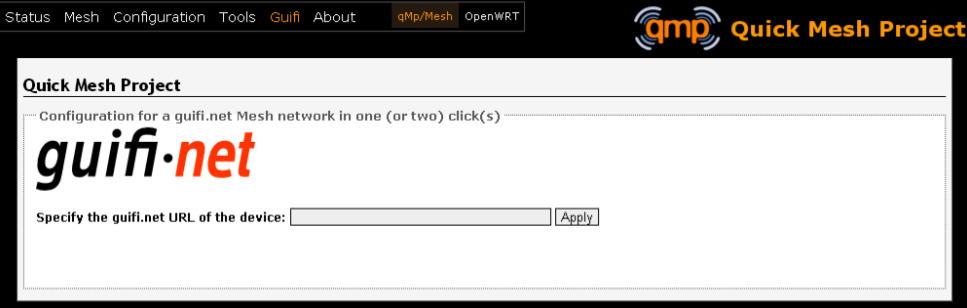
\includegraphics[width=.9\linewidth]{./img/qMp-basics-scrot/qmpguifi.png}
\caption{\label{fig:qmpguifi}guifi.net menu in qMp firmware}
\end{figure}
\subsection{\textbf{munin}:}
\label{sec-11-2}
For a GNU/Linux Debian 7 Wheezy server (apache 2.2)
\begin{verbatim}
sudo apt-get install munin
\end{verbatim}
by default it does monitoring of the server itself (localhost).

For make the graphs available for every user \footnote{Solution for apache 2.2 and 2.4: \url{http://stackoverflow.com/questions/9127802}} in order to follow the
Community Network model of open all network data change the
following lines in \texttt{/etc/munin/apache.conf}:
\begin{verbatim}
Order allow,deny
Allow from localhost 127.0.0.0/8 ::1
Options None
\end{verbatim}
like so:
\begin{verbatim}
Order allow,deny
Allow from all
Options FollowSymLinks SymLinksIfOwnerMatch
\end{verbatim}
Apply the changes in the HTTP server:
\begin{verbatim}
# service apache2 restart
\end{verbatim}

Add qMp nodes for monitor them editing the file \texttt{/etc/munin/munin.conf}:
\begin{verbatim}
[qMp-node1]
    address 10.x.x.x
    use_node_name yes
[qMp-node2]
    address 10.x.x.x
    use_node_name yes
\end{verbatim}

Apply the changes in the monitor (it will start appearing after few
minutes):
\begin{verbatim}
# service munin-node restart
\end{verbatim}
The graphics are very similar to those of guifi, but provide more
information. Except that there is an error with network traffic
monitoring and is not provided.
\subsection{\textbf{qmpsu}:}
\label{sec-11-3}
At the moment, there is not a generic package of qmpsu for qMp networks,
only for Sants Poblenou. More information see
\texttt{Situation of mesh networks in Barcelona}. Figure \ref{fig:qmpsu} shows how it
looks like.

\begin{figure}[htb]
\centering
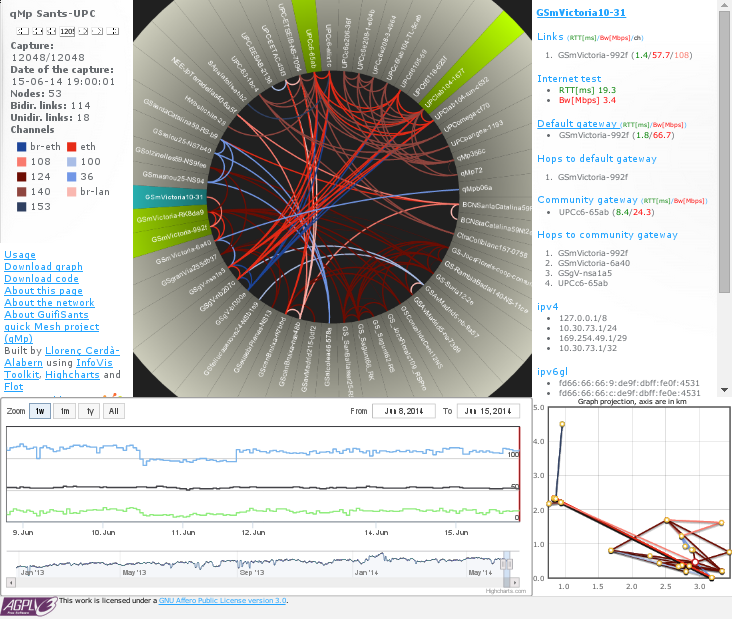
\includegraphics[width=.9\linewidth]{./img/general/qmpsu.png}
\caption{\label{fig:qmpsu}qmpsu view}
\end{figure}
% Emacs 24.4.50.1 (Org mode 8.2.6)
\end{document}
